% !TEX root = main.tex
\documentclass[a4paper, UKenglish, 11pt]{uiomaster}
\usepackage{lipsum}
\usepackage[subpreambles=true]{standalone}
\usepackage[table,xcdraw]{xcolor}

\begin{document}

\chapter{Localizing Single Current Dipole Sources}
\rednote{Here comes the results}
In this chapter we will be looking at DiLoc's performance of the inverse problem. With the use of error metrics such as mean absolute error (MAE), mean euclidean distance (MED) and root mean euclidean distance (RMED) we will study how the DiLoc, as a simple feed forward neural network ables to solve the inverse EEG problem.

% Section 1 deal with the results and discussion of the simple feed forward neural network, while section 2 will discuss how the alternative convolution neural network performe some of the same results.

\section{Testing Methodology}
Upon achieving full training convergence, a neural network is deemed to have successfully discerned relevant patterns within the training dataset and optimized its parameters to minimize the cost function. To assess the performance of DiLoc, we turn our attention to an independent test dataset, encompassing 20,000 samples. This distinct dataset remains entirely unexposed to the network during the training process, serving as an unbiased and objective measure of the model's predictive accuracy and its capacity to generalize effectively to novel, unseen data.

To comprehensively evaluate the predictive capabilities of our DiLoc neural network on the test dataset, we have employed a diverse set of error metrics. Our primary objective is to ensure that DiLoc accurately predicts the locations of current dipoles in the cerebral cortex based on EEG data recorded from randomly distributed sources. Thus, the main focus lies on minimizing the MED as an overarching measure of performance, however we recognize the importance of diving into the performance of specific target coordinates, i.e., the $x$, $y$, and $z$ values.

The MAE offers a straightforward measure of average prediction error for each individual target coordinate. When evaluating the distance between a specific target coordinate (e.g., $x$, $y$, or $z$) and the corresponding predicted value, this metric provides a clear and easily interpretable measure of the accuracy of DiLoc's predictions for each dimension. It allows us to assess whether the network gives precise predictions for all target values or if it exhibits variations in accuracy across different coordinate dimensions.

In contrast, MSE introduces a squaring process that significantly penalizes larger errors across all dimensions. While this aspect helps in emphasizing and addressing significant deviations between the predicted and true coordinates, it presents values in squared units of the target values, which can be less intuitive to deal with when assessing individual coordinate components.

To address the squared unit issue of MSE while still considering error spread, we have incorporated RMSE into our evaluation framework. RMSE balances the emphasis on significant errors while yielding results in units consistent with the target coordinate values, making it more suitable for evaluating individual coordinate predictions (e.g., $x$, $y$, and $z$).

%
% We begin by introducing the standard inverse problem for our neural network, DiLoc. In this context, the standard inverse problem refers to the task of predicting the x-, y-, and z-coordinates of dipole current sources responsible for generating measured EEG signals. The goal is to feed the network with EEG data corresponding to the electrical activity from randomly distributed dipoles in the cerebral cortex and have the network accurately output the locations of these current dipoles.
%

% For this specific problem, the network demonstrates remarkable performance even without the use of L1 regularization. However, we include L2 penalty with a value of 0.5 to promote more generalizable solutions.

\section{Need a name}
According to Ness et al. (2021) \cite{naess2021biophysically}, EEG signals are not particularly sensitive to minor shifts in the precise location of neural current dipoles. This insensitivity can be explained by the fact that relative to the dimensions of individual neurons and the thickness of the human cortex, EEG electrodes are located far away from cortical neural sources. Before commencing the assessment of DiLoc's performance, we aim to investigate whether it has the capability to differentiate EEG signals originating from neighboring neural dipoles and provide distinct predictions for their respective spatial locations. By .... Pearson correlation coefficient ....

The \emph{Pearson correlation coefficient} is a useful statistical measure that quantifies the relationship between two variables. This coefficient is defined as the ratio between the covariance of the two variables and the product of their standard deviations. The coefficient is always a single number within the range of -1 to 1, with -1 denoting a perfect negative correlation and 1 indicating a perfect positive correlation. When the correlation coefficient equals 0, it signifies the absence of a linear relationship between the variables \cite{numpy-docs}.

In our exploration of EEG insensitivity to small differences in dipole locations, we utilize the correlation coefficient as a measure. Figure \ref{fig:neighbour_dipoles} illustrates three EEG signals corresponding to dipoles positioned at neighboring points within the NYHM cortical matrix. The central blue dipole is positioned by the green and red dipoles, situated at the leftmost and rightmost positions within the cortical matrix, respectively. The Euclidean distance between the blue and green dipoles is 0.914 mm, while the blue and red dipoles are separated by 1.926 mm.

The EEG signals of the blue and green dipoles in Figure \ref{fig:neighbour_dipoles} exhibit significant overlap, supported by a high correlation coefficient of 0.966, indicating a strong positive relationship between these measurements. Conversely, the EEG signals of the blue and red dipoles show less resemblance, with a correlation coefficient of 0.695, denoting a somewhat smaller linear relationship. Notably, these differences can be attributed to the rotation in the normal vector of the red dipole and the somewhat larger distance between the blue and red dipoles compared to the blue and green dipoles.

The rotation of the normal vector is also evident for the green dipole but is more pronounced for the red dipole. When selecting neighboring dipoles within the NYHM based on distance, rotations in the normal vectors occur due to constraints during data generation that ensure dipole orientation is perpendicular to the cerebral cortex. Given the complex folding of the cortex, such constraints may lead to rotations in the dipole normal vector when shifting the dipole's location, as demonstrated in this example. Consequently, distinct differences in simulated EEG signals may emerge even for neighboring dipoles within the NYHM.

%Despite the common belief that neurons in the upper cortical layers would dominate the EEG due to their proximity to the electrode compared to neurons in deeper layers, such location differences do not significantly affect the EEG signals. This phenomenon can be explained by the fact that the low conductivity of the skull introduces a spatial low-pass filtering effect, which mitigates the impact of location discrepancies.
% Maybe what is meant here is that we therefore only consider the outer corical surface

\begin{figure}[!htb]
    \centering
    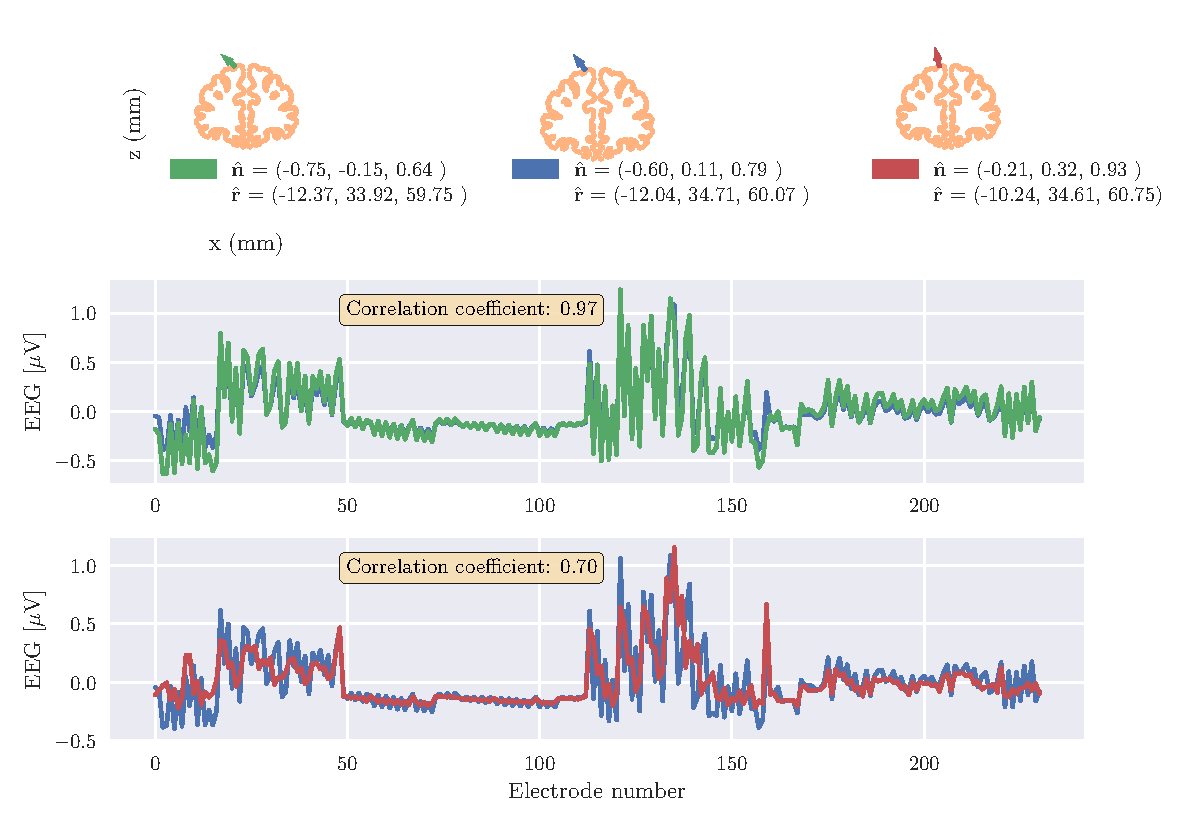
\includegraphics[width=\linewidth]{figures/compare_dipoles.pdf}
    \caption{EEG signals plotted against electrode number for three neighbouring dipoles with normal vectors (-0.60, 0.11, 0.79), (-0.75, -0.15, 0.64), (-0.21, 0.32, 0.93) and positions (-12.04, 34.71, 60.07), (-12.37, 33.92, 59.75), (-10.24, 34.61, 60.75). The correlation coefficient between the blue and green dipole is 0.97, while it is 0.70 for the blue and red dipole. \rednote{Which coordinate system? Where is (0,0,0) located?}}
    \label{fig:neighbour_dipoles}
\end{figure}


\section{Performance Evaluation}
The neural network was trained for 500 epochs, with MED loss convergence depicted in Figure \ref{fig:single_dipole_accuracy}. The training time for one epoch was approximately 11.00 seconds, summing up to a total training time of 5500 seconds, equivalent to roughly 1.5 hours. It's important to note that this training duration does not include data loading and preprocessing.

The validation loss appeared to stabilize after approximately 350 epochs. At this point, the training could have been stopped. However, we extended the training to the full 500 epochs. This decision was made to confirm that no further improvements in the validation data's performance would occur and to emphasize that the network had fully converged when undergoing evaluation.

Figure \ref{fig:single_dipole_accuracy} illustrates a clear trend of decreasing loss, indicating that the network effectively learned patterns in the data. The validation loss stabilization is noticeable around 350 epochs, while the training loss continues to decrease until it stabilizes between 400 and 500 epochs. This observation suggests that the model did not exhibit signs of overfitting, as the validation loss remained constant, and the training loss eventually stabilized.

Additionally, Figure \ref{fig:single_dipole_accuracy_targets} provides insight into the development of the validation loss for the separate target coordinates, $x$, $y$, and $z$, plotted against training epochs. This figure confirms that all separate target coordinates were equally weighted, resulting in similar loss values for each. Moreover, it demonstrates that the small fluctuations in loss, observed before 350 epochs, disappeared beyond this threshold, indicating a stabilization of the loss for all three target coordinates. This observation aligns with the trend of the validation loss stabilizing at approximately 350 epochs, that we could see in Figure \ref{fig:single_dipole_accuracy}.

\begin{figure}[!htb]
    \centering
    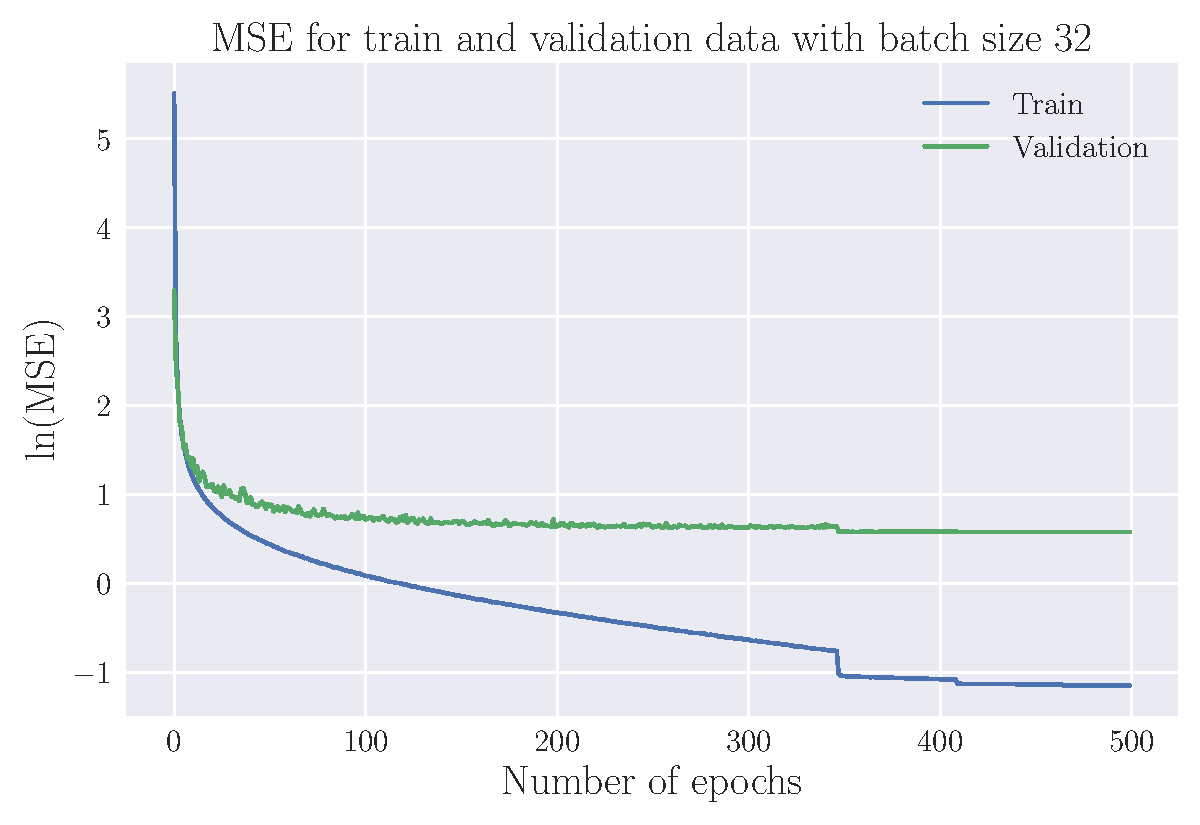
\includegraphics[width=\linewidth]{figures/mse_simple_32_0.001_0.35_0.5_0.0_500_(0).pdf}
    \caption{Training- and validation MED loss for DiLoc with 50,000 samples and tanh as activation function.}
    \label{fig:single_dipole_accuracy}
\end{figure}

\begin{figure}[!htb]
    \centering
    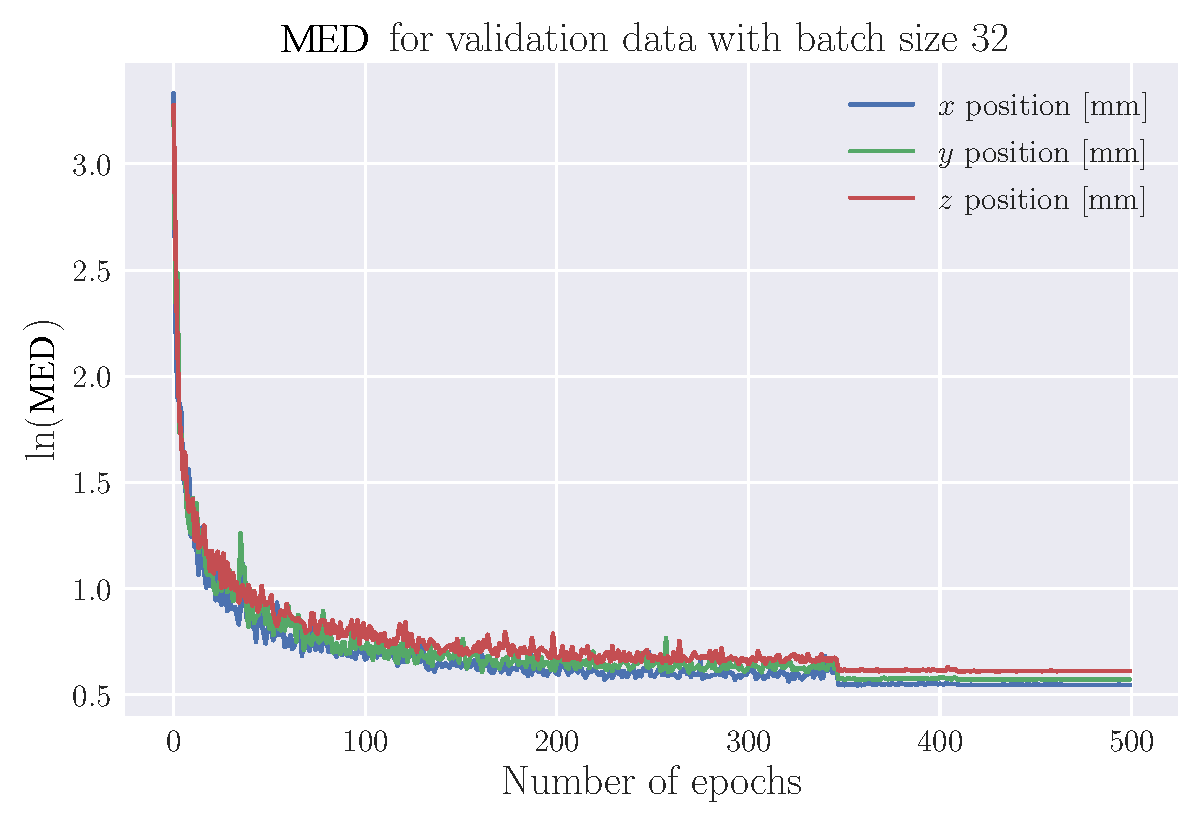
\includegraphics[width=\linewidth]{figures/mse_targets_simple_32_0.001_0.35_0.5_0.0_500_(0).pdf}
    \caption{Validation MED loss for the separate target values; the $x$-, $y$-, $z$-coordinate.}
    \label{fig:single_dipole_accuracy_targets}
\end{figure}


\subsection{Position Spesific Performance}
\rednote{Range of values should be placed somewhere else. Errors should be contextualized within the range.}
In evaluating the DiLoc network's performance, we further examined its accuracy across three spatial coordinates: $x$, $y$, and $z$. These coordinates represent the positions of dipole sources in three-dimensional space. Notably, the $x$-coordinate ranges from -72 to 72 mm, the $y$-coordinate from -106 to 73 mm, and the $z$-coordinate from -53 to 82 mm, providing context for the interpretation of error metrics.

\rednote{Add histogram instead of table?}
The MED of DiLoc's predictions on the unseen test data measures 1.33 mm. In Table \ref{table:MED}, we have provided the percentages of samples falling within various MED threshold values. Impressively, DiLoc provides an accuracy smaller than 12 mm for the entirety of the samples within the test dataset. Furthermore, it is noteworthy that an impressive 96.6$\%$ of the samples exhibit a MED smaller than 3 mm, an achievement that underscores the network's high precision.

% Please add the following required packages to your document preamble:
% \usepackage[table,xcdraw]{xcolor}
% If you use beamer only pass "xcolor=table" option, i.e. \documentclass[xcolor=table]{beamer}
\begin{table}[]
\begin{tabular}{|cccl|}
\hline
\rowcolor[HTML]{CBCEFB}
\multicolumn{4}{|c|}{\cellcolor[HTML]{CBCEFB}\textbf{Mean Euclidian Distance for Test Samples}}                                                                                                                                                                 \\ \hline
\rowcolor[HTML]{EFEFEF}
\multicolumn{1}{|c|}{\cellcolor[HTML]{EFEFEF}MED \textless 3 mm} & \multicolumn{1}{c|}{\cellcolor[HTML]{EFEFEF}MED \textless 5 mm} & \multicolumn{1}{c|}{\cellcolor[HTML]{EFEFEF}MED \textless 10 mm} & MED \textless 12 mm                                     \\ \hline
\rowcolor[HTML]{FFFFFF}
\multicolumn{1}{|c|}{\cellcolor[HTML]{FFFFFF}96.595 $\%$}        & \multicolumn{1}{c|}{\cellcolor[HTML]{FFFFFF}99.735 $\%$}        & \multicolumn{1}{c|}{\cellcolor[HTML]{FFFFFF}99.995 $\%$}         & \multicolumn{1}{c|}{\cellcolor[HTML]{FFFFFF}100.000$\%$} \\ \hline
\end{tabular}
\caption{\textbf{MED evaluation on test samples; Predicting Location} \newline
Performance of the network on thes test dataset comprising 20,000 samples, presented as the percentage of samples falling within MED thresholds of 3 mm, 5 mm, 10 mm, and 12 mm, respectively.}
\label{table:MED}
\end{table}

Table \ref{table:error_simple_dipole} below presents the results for the MAE in the DiLoc network's predictions. Notably, the MAE values for the $x$, $y$, and $z$-coordinates range from 0.645 mm to 0.678 mm. These findings indicate that, on average, the network's predictions exhibit an error smaller than 1 mm in each coordinate, underscoring its high level of accuracy.

The MSE values, ranging from 0.747 mm$^2$ to 0.824 mm$^2$, corroborate the network's remarkable precision. Smaller MSE values signify high performance, and in this evaluation, all MSE values are comfortably below the 1 mm$^2$ threshold. This observation highlights the network's precision, especially given the wide range of coordinates involved. The small MSE values indicate minimal error spread, implying few significant deviations between predicted and true coordinates.

To quantify the accuracy further, RMSE values were computed, ranging from 0.864 mm to 0.908 mm. It is worth noting that RMSE is slightly higher than the corresponding MSE values due to the square root operation involved. Importantly, all RMSE values remain below the 1 mm threshold, signifying that DiLoc's predictions maintain a limited error spread, typically staying within 1 millimeter of the actual values.

To provide overall positional errors given the MAE, MSE, and RMSE, the mean of each error metric is also given in the table. The resulting error values remain small, further reaffirming the network's precision in predicting dipole locations for the inverse problem.

Notably, among the three coordinates, the $z$-coordinate exhibits the highest error values. This observation suggests that the DiLoc network encounters greater challenges in accurately predicting the $z$-coordinate of the dipole source. One plausible explanation is related to the nature of the inverse problem, where the depth of the dipole sources primarily influences the magnitude rather than the pattern of EEG recordings. Additionally, the $z$-coordinate's smaller representation compared to the $x$- and $y$-coordinates could contribute to the consistently larger errors in the $z$-direction. However, we underscore that this discrepancy in error magnitude is very small and could also be influenced by randomness. Overall, these error metrics indicate that the DiLoc network can predict dipole locations with a reasonable level of accuracy.

\rednote{Make figure to show. Mention the practical significance of the example, such as how close the predicted values need to be for specific applications.}
To showcase the networks performance, we look the prediction of a randomly chosen sample within the test set. For a dipole located at $x$ = 66.9 mm, $y$ = -26.1 mm and $z$ = 41.7 mm the network predicts the coordinates to be $x_{\text{pred}}$ = 66.5 mm, $y_{\text{pred}}$ = -26.4 mm and $z_{\text{pred}}$ =  41.9 mm. The predicted values are considerable close to the true values, with an error of 0.4 mm in the $x$-coordinate, 0.3 mm in the $y$-coordinate, and 0.2 mm in the $z$-coordinate, giving an eucleadian distance of 0.54 mm.

% Please add the following required packages to your document preamble:
% \usepackage[table,xcdraw]{xcolor}
% If you use beamer only pass "xcolor=table" option, i.e. \documentclass[xcolor=table]{beamer}
\begin{table}[!htb]
\begin{tabular}{l|cccc|}
\cline{2-5}
\rowcolor[HTML]{CBCEFB}
\cellcolor[HTML]{FFFFFF}                           & \multicolumn{4}{c|}{\cellcolor[HTML]{CBCEFB}{\color[HTML]{000000} \textbf{Error Metrics for Target Values}}}                                                                                                                                                                                                                                                                                                                                                     \\ \cline{2-5}
\rowcolor[HTML]{EFEFEF}
\cellcolor[HTML]{FFFFFF}\textbf{}                  & \multicolumn{1}{l|}{\cellcolor[HTML]{EFEFEF}\begin{tabular}[c]{@{}l@{}}x-coordinate\\ {[}mm{]}\end{tabular}} & \multicolumn{1}{l|}{\cellcolor[HTML]{EFEFEF}\begin{tabular}[c]{@{}l@{}}y-coordinate \\ {[}mm{]}\end{tabular}} & \multicolumn{1}{l|}{\cellcolor[HTML]{EFEFEF}\begin{tabular}[c]{@{}l@{}}z-coordinate \\ {[}mm{]}\end{tabular}} & \multicolumn{1}{l|}{\cellcolor[HTML]{EFEFEF}\begin{tabular}[c]{@{}l@{}}Position \\ Error {[}mm{]}\end{tabular}} \\ \hline
\multicolumn{1}{|l|}{\cellcolor[HTML]{EFEFEF}MAE}  & \multicolumn{1}{c|}{0.645}                                                                                  & \multicolumn{1}{c|}{0.665}                                                                                   & \multicolumn{1}{c|}{0.678}                                                                                   & 0.662                                                                                                              \\ \hline
\multicolumn{1}{|l|}{\cellcolor[HTML]{EFEFEF}MSE}  & \multicolumn{1}{c|}{0.747}                                                                                  & \multicolumn{1}{c|}{0.775}                                                                                   & \multicolumn{1}{c|}{0.824}                                                                                   & 0.782                                                                                                              \\ \hline
\multicolumn{1}{|l|}{\cellcolor[HTML]{EFEFEF}RMSE} & \multicolumn{1}{c|}{0.864}                                                                                  & \multicolumn{1}{c|}{0.880}                                                                                   & \multicolumn{1}{c|}{0.908}                                                                                   & 0.884                                                                                                              \\ \hline
\end{tabular}
\caption{\textbf{Evaluation of the DiLoc performance utializing different Error Metrics.} \newline
Network performance on test dataset consisting of 20000 samples. The errors are measured using Mean Squared Error (MSE), Mean Absolute Error (MAE), and Root Mean Squared Error (RMSE).}
\label{table:error_simple_dipole}
\end{table}

\subsection{Performance at Different Brain Structures}

In order to conduct a further detailed analysis of the network's performance, Figure \ref{fig:MED_crossections} presents the Mean Eucleadian Distance for various dipole locations within the New York head model cortex matrix. The figure provides valuable insights into the distribution of errors across different regions of the cortex, with three cross-sections — front, top, and side — depicted for examination. It is important to note that these cross-sections unavoidably include data points from the training, validation, \emph{and} test datasets, making these results indicative of the network's overall performance rather than real-world scenarios. However, the analysis aims to examine the distribution of errors and identify potential areas where the network's performance may be weaker, helping to gain valuable insights into its predictive capabilities.

The MED values presented in the panels are mostly below 1 mm, which indicates a high level of accuracy in the network's predictions. These results are promising and demonstrate the network's ability to estimate dipole locations with a high level of precision. The panels also offer an opportunity to assess whether the network performs differently for dipoles located in the gyrus compared to the sulcus.

Initially, it might be assumed that EEG signals originating from dipoles in the sulcus present greater challenges for the network's analysis and prediction. This assumption is based on the deeper placement of dipoles within the sulcus compared to those in the gyrus, as well as the potential complexities introduced by the dipole's orientation within the cortex. However, upon closer examination of Figure \ref{fig:MED_crossections}, it becomes evident that the distribution of MED values does not exhibit a clear correlation with the brain's structural characteristics. The MED values appear to vary randomly across different regions, indicating that the network's performance is not significantly influenced by the distinction between the gyrus and sulcus.

Surprisingly, the Mean Euclidian Distance (MSE) for all data points where dipoles are located in sulci is measured to be 1.68 mm, which is even smaller than for dipoles in the gyrus, where the MSE measures 1.70 mm. This observation challenges the initial assumption, and rather indicates that the network demonstrates exceptional accuracy in predicting dipole locations, irrespective of their placement within the cortex. The small MED values further underscore the network's remarkable capacity to effectively capture the intricate features and variations associated with deeper cortical placements. These findings not only attest to the network's robustness but also reinforce its potential for precise dipole localization within the human brain across different cortical structures.

\rednote{The "theory" should be mentioned somewhere else and already be known for the reader.}
Furthermore, the figures reveal a somewhat noticeable concentration of data points with red marks in the deeper locations within the cortex, indicating higher MED values. This observation is consistent with the slightly higher error values observed for the z-coordinate, as presented in Table \ref{table:error_simple_dipole}, and aligns with the theory related to the nature of the inverse problem. According to this theory, EEG patterns for dipole sources do not cause substantial changes in the pattern of electrical potential recordings; instead, they primarily influence the magnitude of the signals, which may challenge DiLoc's ability to discriminate deep sources from each other. Said with other words, the presence of higher MED values in deeper regions might be attributed to the decreasing signal-to-noise ratio of EEG signals originating from these cortical areas.

In conclusion, the detailed analysis of the network's performance through cross-sectional representations provides valuable insights into its predictive capabilities. The consistently low MED across different cortical regions demonstrate the network's remarkable accuracy in estimating dipole locations. Moreover, the absence of a clear correlation between MED and brain structural characteristics suggests that the network performs robustly across diverse cortical structures. These results have significant implications for the network's potential clinical and research applications, as it showcases its ability to accurately predict dipole locations within the human brain, regardless of their depth and orientation within the cortex.

\begin{figure}[!htb]
    \centering
    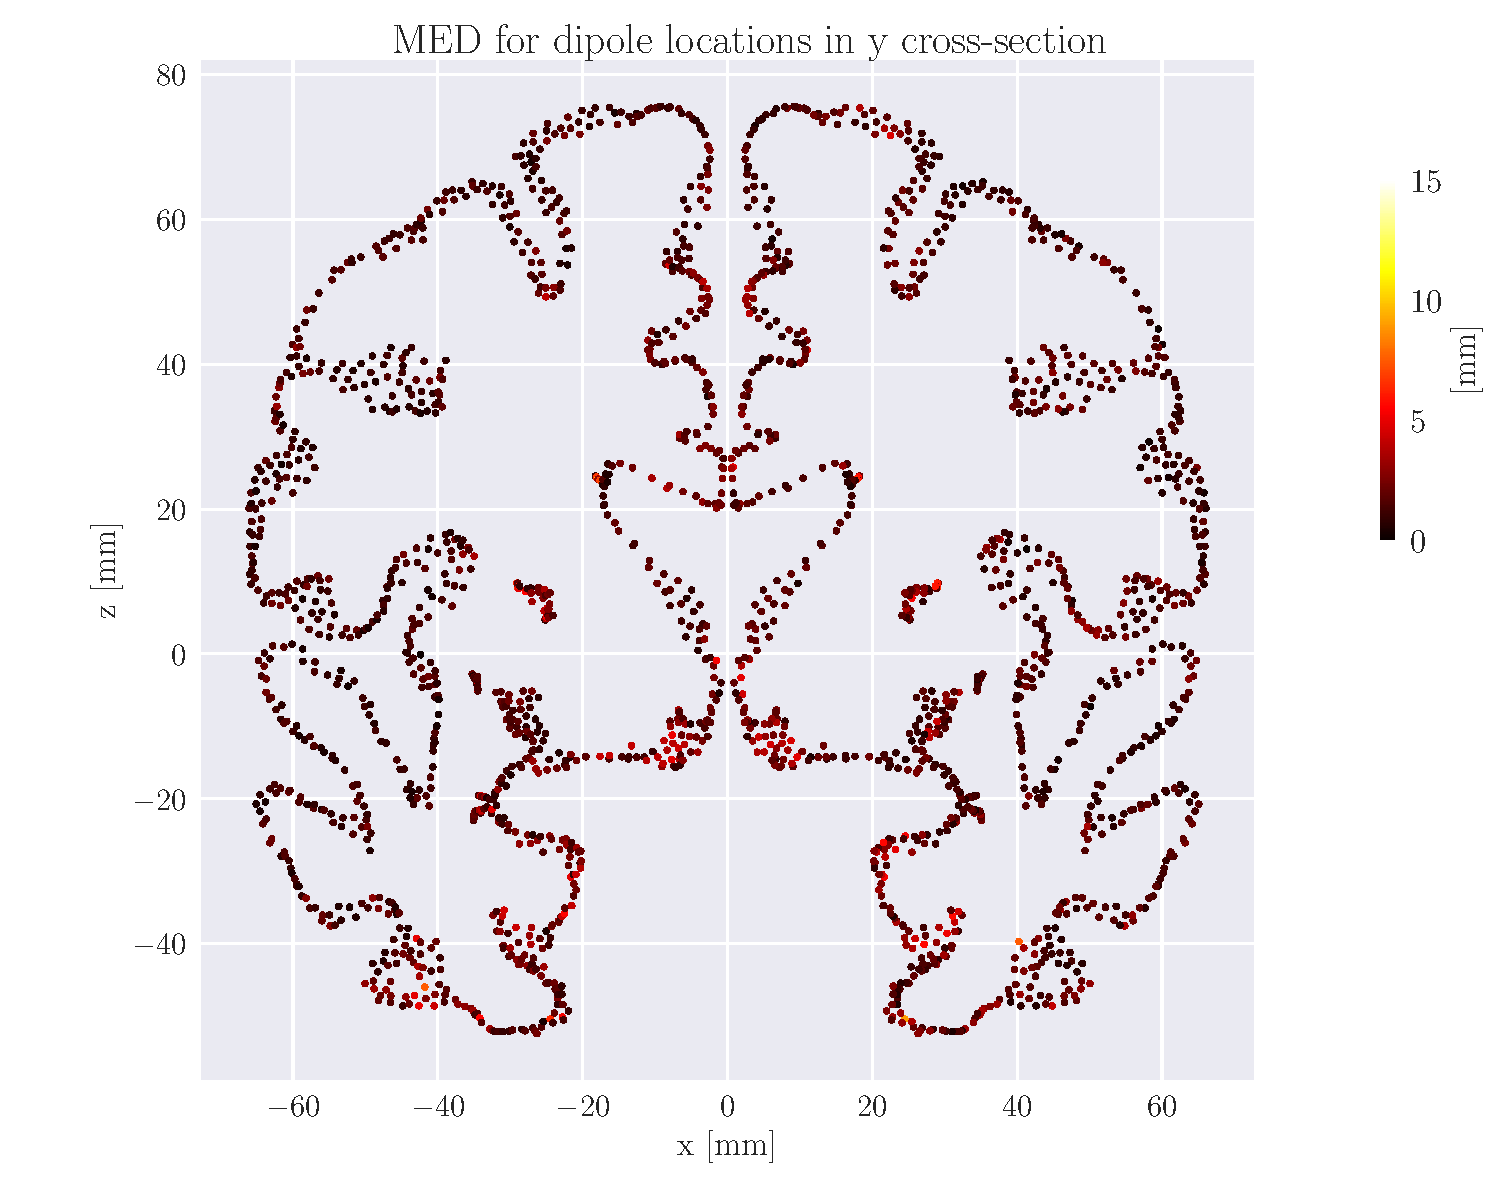
\includegraphics[width=0.7\linewidth]{figures/MED_simple_dipole_error_Euclidean Distance_0.pdf}
    \vspace{10pt} % Adjust the vertical spacing between the images
    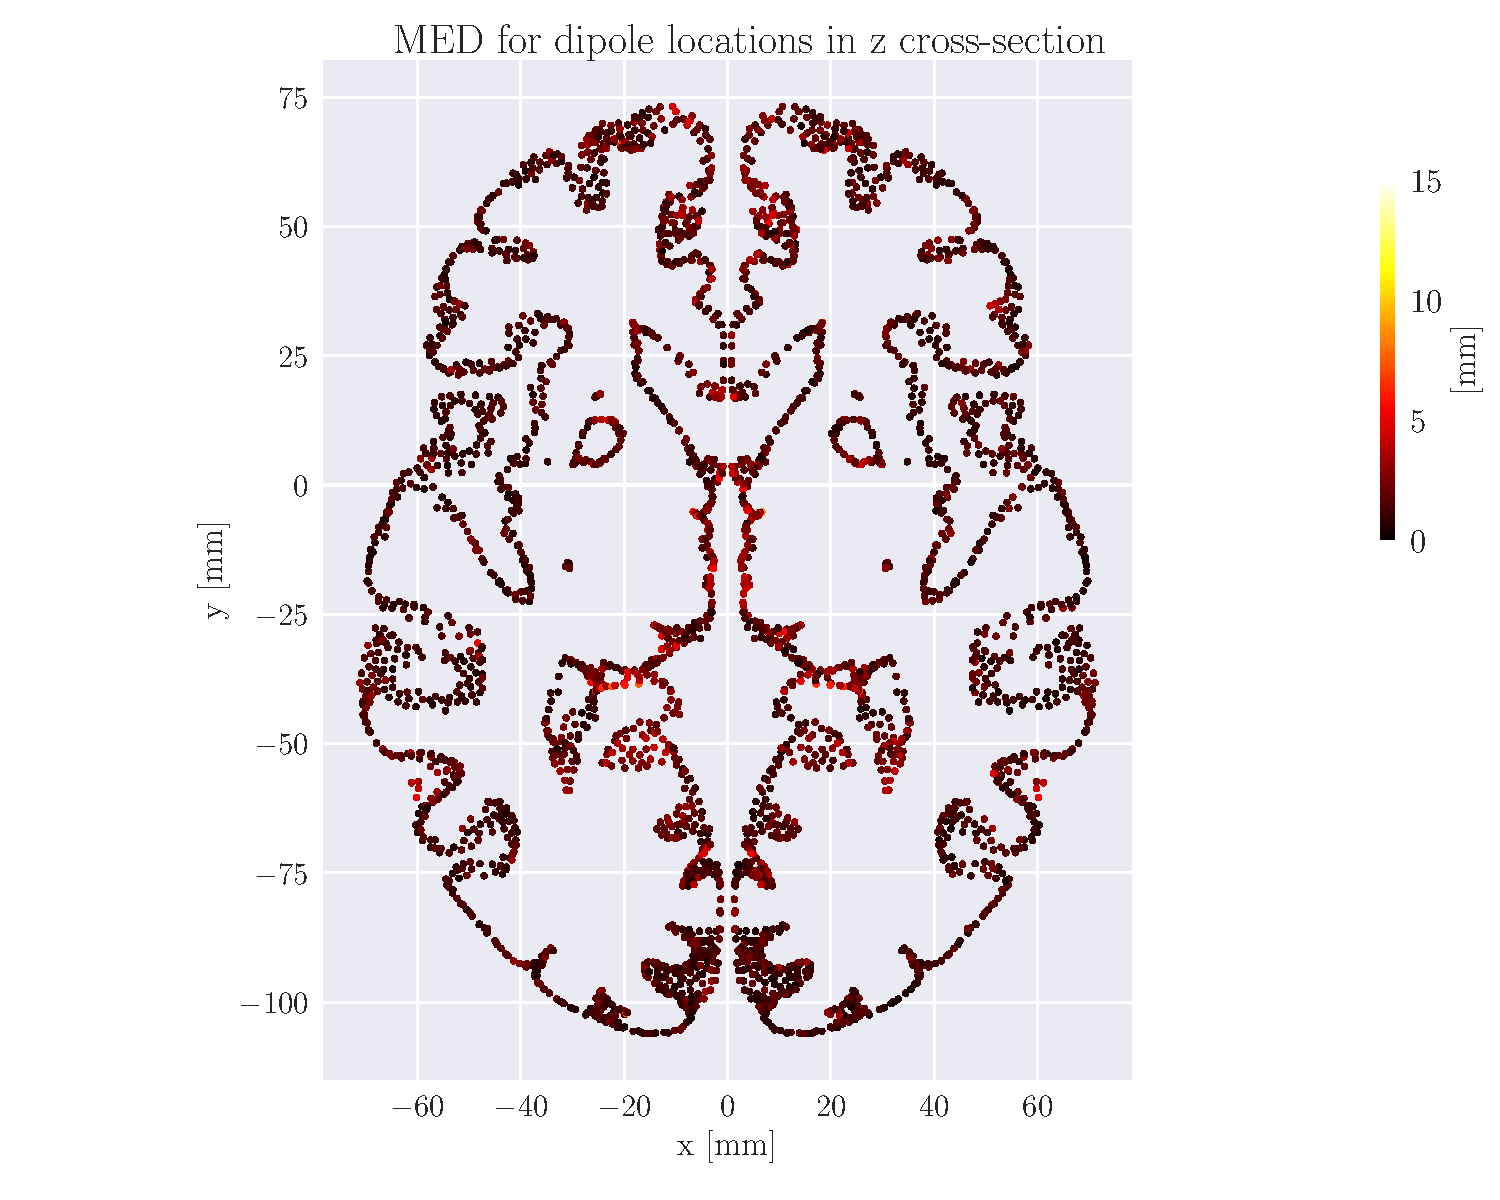
\includegraphics[width=0.7\linewidth]{figures/MED_simple_dipole_error_Euclidean Distance_1.pdf}
    \vspace{10pt} % Adjust the vertical spacing between the images
    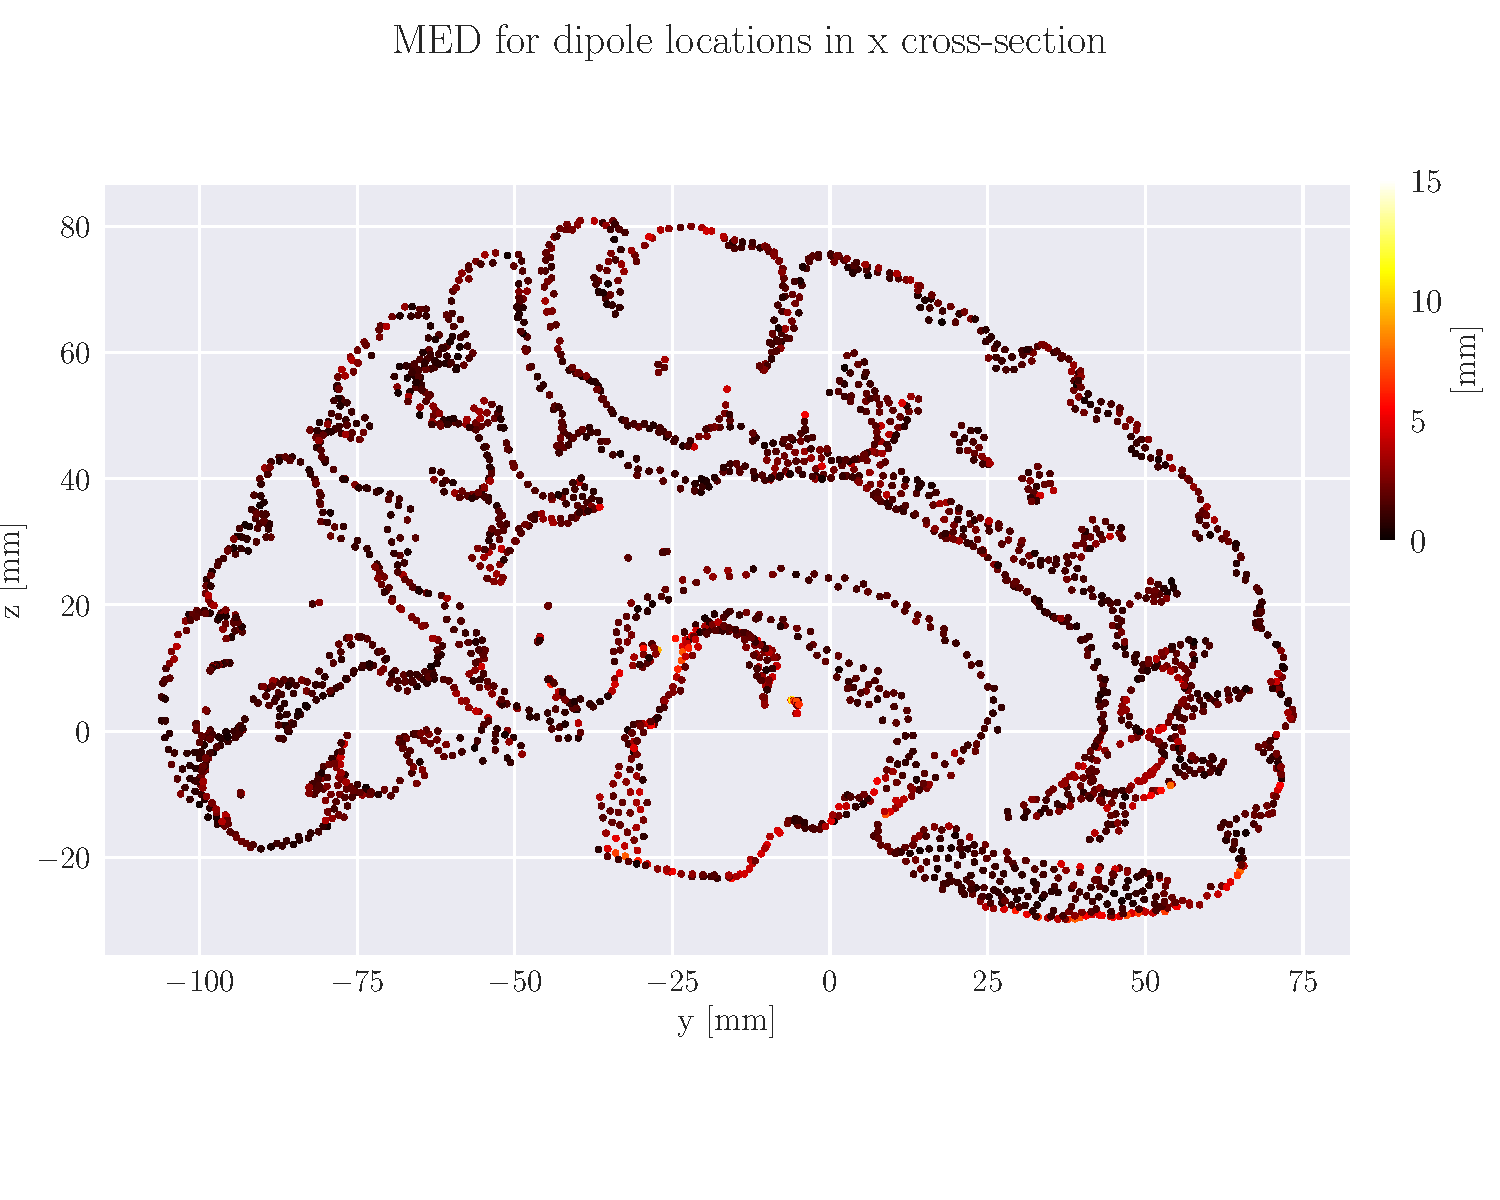
\includegraphics[width=0.7\linewidth]{figures/MED_simple_dipole_error_Euclidean Distance_2.pdf}
    \caption{Different cross-sections of the cortex from the New York head model, seen from front, top and side. Each point represents a possible position in the cortex matrix. The color of the each point indicates the mean absolute error (MAE) of the neural network when predicting that specific dipole location.}
    \label{fig:MED_crossections}
\end{figure}



\end{document}
